% !TeX program = lualatex
% !TeX encoding = utf8
% !TeX spellcheck = uk_UA
% !TeX root =../MexPractEng.tex

%=========================================================
\chapter{Dynamics. Newtonian laws}\label{\currfilebase}
\Opensolutionfile{answer}[\currfilebase/\currfilebase-Answers]
\Writetofile{answer}{\protect\section*{\nameref*{\currfilebase}}}%
%=========================================================

\section{Applying Newton’s Laws}


%=========================================================
\begin{problem}\label{prb:Mass_on_cord}
	In Fig.~\ref{Mass_on_cord}, let the mass of the block be $m = 8.5$~\si{\kilo\gram} and the angle be $\alpha = \ang{30}$.
	Find 
	\begin{enumerate*}[label = (\alph*)]
		\item the tension in the cord and
		\item the normal force acting
		on the block.
		\item If the cord is
		cut, find the magnitude of the resulting acceleration of the block.
	\end{enumerate*}
\end{problem}


%=========================================================
\begin{problem}\label{prb:ramp}
	In Fig.~\ref{Mass_on_cord} a crate of mass $m = 100$~\si{\kilo\gram} is pushed at constant velocity up a frictionless ramp
	($\alpha = \ang{30.0}$) by a horizontal force. What are the magnitudes of 
		\begin{enumerate*}[label = (\alph*)]
		\item force $\vec F$ and
		\item the force on the crate from the ramp?
	\end{enumerate*}
\end{problem}


%=========================================================
\begin{figure}[h!]\centering
	%---------------------------------------------------------
	\begin{minipage}[t]{0.45\linewidth}\centering
		\begin{tikzpicture}
			\tikzstyle{ground}=[fill,pattern=north east lines,draw=none,minimum width=2cm,minimum height=0.3cm]
			\pgfmathsetmacro{\h}{3}
			\pgfmathsetmacro{\l}{4}
			\pgfmathsetmacro{\incangle}{atan(\h/\l)}
			\node (wall) at (\l,\h/2 + 1) [rotate=90, ground, minimum width=\h cm + 2cm,yshift=-0.15cm] {};
			\draw (wall.north west) -- (wall.north east);
			\fill[brown!50, draw=black] (0,0) -- ++(\l,0) -- ++(0,\h) coordinate(A) -- cycle;
			\draw[-latex] (0,0) +(0:0.5) arc (0:\incangle:0.5) node[pos=0.5, right] {$\alpha$};
			\path (0,0) -- (A) coordinate[pos=0.3] (B);
			\draw[fill=green!50, rotate=\incangle] (B) rectangle  +(1,1) [add reference=BP1];
			\node[rotate=\incangle] at (BP1 center) {$m$};
			\draw[red, ultra thick] (BP1 east) -- (\l,{\h+0.5/(cos(\incangle))}) node[pt=blue] {};
		\end{tikzpicture}
		\caption{Problem~\ref{prb:Mass_on_cord}}
		\label{Mass_on_cord}
	\end{minipage}
	%---------------------------------------------------------
	\begin{minipage}[t]{0.45\linewidth}\centering
		\begin{tikzpicture}
			\pgfmathsetmacro{\h}{3}
			\pgfmathsetmacro{\l}{4}
			\pgfmathsetmacro{\incangle}{atan(\h/\l)}
			\fill[brown!50, draw=black] (0,0) -- ++(\l,0) -- ++(0,\h) coordinate(A) -- cycle;
			\draw[-latex] (0,0) +(0:0.5) arc (0:\incangle:0.5) node[pos=0.5, right] {$\alpha$};
			\path (0,0) -- (A) coordinate[pos=0.3] (B);
			\draw[fill=green!50, rotate=\incangle] (B) rectangle  +(1,1) [add reference=BP1];
			\draw[-latex, thick, double, blue] (BP1 center) -- +(2,0) node[right] {$\vec F$};
		\end{tikzpicture}
		\caption{Problem~\ref{prb:ramp}}
		\label{ramp}
	\end{minipage}
	%---------------------------------------------------------
\end{figure}
%=========================================================
%=========================================================
\begin{problem}\label{prb:Athwood}
	Two blocks connected by a cord (of negligible mass) that passes over a frictionless
	pulley (also of negligible mass) (see Fig.~\ref{Athwood}). The arrangement is known as \textit{Atwood's machine}. One
	block has mass $m_1 = 1.30$~\si{\kilo\gram}; the other has mass $m_2 =
	2.80$~\si{\kilo\gram}. What are 
	\begin{enumerate*}[label = (\alph*)]
		\item the magnitude of the blocks' acceleration
		\item and the tension in the cord?
	\end{enumerate*}
%---------------------------------------------------------
\end{problem}

%=========================================================
\begin{figure}[h!]\centering
	%---------------------------------------------------------
	\begin{minipage}[t]{0.45\linewidth}\centering
		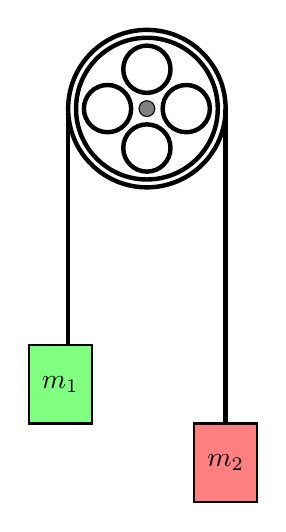
\begin{tikzpicture}
		\draw[ultra thick, fill=white] (0.0,10) circle (1);
		\draw[ultra thick] (0.0,10) circle (0.9);
		\draw[ultra thick] (-0.5,10) circle (0.3);
		\draw[ultra thick] (0.5,10) circle (0.3);
		\draw[ultra thick] (0,10.5) circle (0.3);
		\draw[ultra thick] (0,9.5) circle (0.3);
		\draw[fill=gray] (0.0,10) circle (0.1);
		\draw[ultra thick] (-1,10) -- (-1,7);
		\draw[thick, fill=green!50] (-1.5,7) rectangle node {$m_1$} +(0.8,-1);
		\coordinate (B) at (1,6);
		\draw[ultra thick] (1,10) --  (B);
		\draw[thick, fill=red!50] ([shift={(-0.4,0)}]B) rectangle node {$m_2$} +(0.8,-1);
		\end{tikzpicture}
		\caption{Problem~\ref{prb:Athwood}}
		\label{Athwood}
	\end{minipage}
	%---------------------------------------------------------
	\begin{minipage}[t]{0.45\linewidth}\centering
		\begin{tikzpicture}
			\pgfmathsetmacro{\h}{3}
			\pgfmathsetmacro{\l}{4}
			\pgfmathsetmacro{\incangle}{atan(\h/\l)}
			\pgfmathsetmacro{\R}{0.5}
			\coordinate (R) at (\incangle:5.5);
			\fill[brown!50, draw=black] (0,0) -- ++(\l,0) -- ++(0,\h) coordinate(A) -- cycle;
			\draw[-latex] (0,0) +(0:0.5) arc (0:\incangle:0.5) node[pos=0.5, right] {$\alpha$};
			\coordinate (RT1) at  ([shift={(135:\R)}]R);
			\coordinate (RT2) at  ([shift={(0:\R)}]R);
			\draw[fill=gray, thick] (R) circle (\R)
			circle (\R-0.1)
			circle (0.05);
			\path (0,0) -- (A) coordinate[pos=0.3] (B);
			\draw[fill=green!50, rotate=\incangle] (B) rectangle  +(1,1) [add reference=BP1];
			\draw (BP1 east) -- (RT1);
			\draw[fill=red!50] ([shift={(-0.5,-3)}]RT2) rectangle  +(1,1) [add reference=BP2];
			\draw (BP2 north) -- (RT2);
			\node[rotate=\incangle] at (BP1 center) {$m_1$};
			\node[] at (BP2 center) {$m_2$};
		\end{tikzpicture}
		\caption{Problem~\ref{prb:inc}}
		\label{inc}
	\end{minipage}
	%---------------------------------------------------------
\end{figure}
%=========================================================


%=========================================================
\begin{problem}\label{prb:inc}
	A block of mass $m_1 = 3.70$~\si{\kilo\gram} on a frictionless plane inclined
	at angle $\alpha = \ang{30.0}$ is connected by a cord over a massless,
	frictionless pulley to a second block of mass $m_2 = 2.30$~\si{\kilo\gram} (Fig.~\ref{inc}). What are 
	\begin{enumerate*}[label = (\alph*)]
		\item he magnitude of the acceleration of each block,
		\item he direction of the acceleration of the hanging block,
		\item the tension in the cord?
	\end{enumerate*}
\end{problem}


%=========================================================
\begin{problem}\label{prb:Blocks}
	In Fig.~\ref{Blocks1}, a constant horizontal force is applied to block $A$, which pushes against block B with a $20.0$~\si{\newton} force directed horizontally to the right. In Fig.~\ref{Blocks2}, the same force is applied
	to block B; now block A pushes on block B with a $10.0$~\si{\newton}  force directed horizontally to the left.The blocks have a combined mass of $12$~\si{\kilo\gram}. What are the magnitudes of
	\begin{enumerate*}[label = (\alph*)]
		\item their acceleration in Fig.~\ref{Blocks1}
		\item and force $\vec F$?
	\end{enumerate*}
\begin{solution}
	\begin{enumerate*}[label = (\alph*)]
	\item $a = 2.5$~\si{\meter\per\square\second}
	\item and $F = 30$~\si{\newton}.
	\end{enumerate*}	
\end{solution}
\end{problem}

%=========================================================
\begin{figure}[h!]\centering
	%---------------------------------------------------------
	\begin{subfigure}[t]{0.3\linewidth}\centering
				\begin{tikzpicture}
					\tikzstyle{ground}=[fill,pattern=north east lines,draw=none,minimum width=2cm,minimum height=0.3cm]
					\node (wall1) [ground, minimum width=5cm,yshift=-0.15cm] {};
					\draw (wall1.north west) -- (wall1.north east);
					\fill[red!50, draw=black] (-1,0) rectangle +(1,1) [add reference=AP];
					\fill[green!50, draw=black] (0,0) rectangle +(1,2) [add reference=BP];
					\draw[-{Latex[open]}, thick, double distance=1pt] (-2,0.5) -- node[above] {$\vec F$} +(1,0);
					\node at (AP center) {A}; \node at (BP center) {B};
				\end{tikzpicture}
		\caption{}
		\label{Blocks1}
	\end{subfigure}
	%---------------------------------------------------------
	\begin{subfigure}[t]{0.3\linewidth}\centering
				\begin{tikzpicture}
				\tikzstyle{ground}=[fill,pattern=north east lines,draw=none,minimum width=2cm,minimum height=0.3cm]
				\node (wall1) [ground, minimum width=5cm,yshift=-0.15cm] {};
				\draw (wall1.north west) -- (wall1.north east);
				\fill[red!50, draw=black] (0,0) rectangle +(1,1) [add reference=AP];
				\fill[green!50, draw=black] (-1,0) rectangle +(1,2) [add reference=BP];
				\draw[-{Latex[open]}, thick, double distance=1pt] (-2,0.5) -- node[above] {$\vec F$} +(1,0);
				\node at (AP center) {A}; \node at (BP center) {B};
				\end{tikzpicture}
		\caption{}
		\label{Blocks2}
	\end{subfigure}
	\caption{Problem~\ref{prb:Blocks}}
	%---------------------------------------------------------
\end{figure}
%=========================================================


%=========================================================
\begin{problem}
	A lamp hangs vertically from a cord in a descending elevator that decelerates at $2.4$~\si{\meter\per\square\second}. 
	\begin{enumerate*}[label = (\alph*)]
		\item If the tension in the cord is $89$~\si{\newton}, what is the lamp’s mass?
		\item What is the cord’s tension when the elevator ascends with an upward acceleration of $2.4$~\si{\meter\per\square\second}?
	\end{enumerate*}
\end{problem}



%=========================================================
\begin{problem}\label{prb:ramp2}
	A box of mass $5.00$~\si{\kilo\gram}, is sent sliding up a frictionless ramp at an angle of $\alpha$ to the horizontal. Fig.~\ref{ramp2}, as a function of time $t$, the component $v_x$ of the box's velocity along an
	$x$ axis that extends directly up the ramp. What is the magnitude of the normal force on the box from the ramp?
\end{problem}

%=========================================================


%=========================================================
\begin{problem}\label{prb:block_friction}
	A $3.5$~\si{\kilo\gram} block is pushed along a horizontal floor by a force of magnitude $15$~\si{\newton} at an angle \ang{40} with the horizontal (Fig.~\ref{block_friction}). The coefficient of kinetic friction between the block and the floor is $0.25$. Calculate the magnitudes of 
	\begin{enumerate*}[label = (\alph*)]
		\item the frictional force on the block from the floor and
		\item the block's acceleration.
	\end{enumerate*}
\end{problem}


\begin{figure}[h!]\centering
	%---------------------------------------------------------
	\begin{minipage}[t]{0.45\linewidth}\centering
			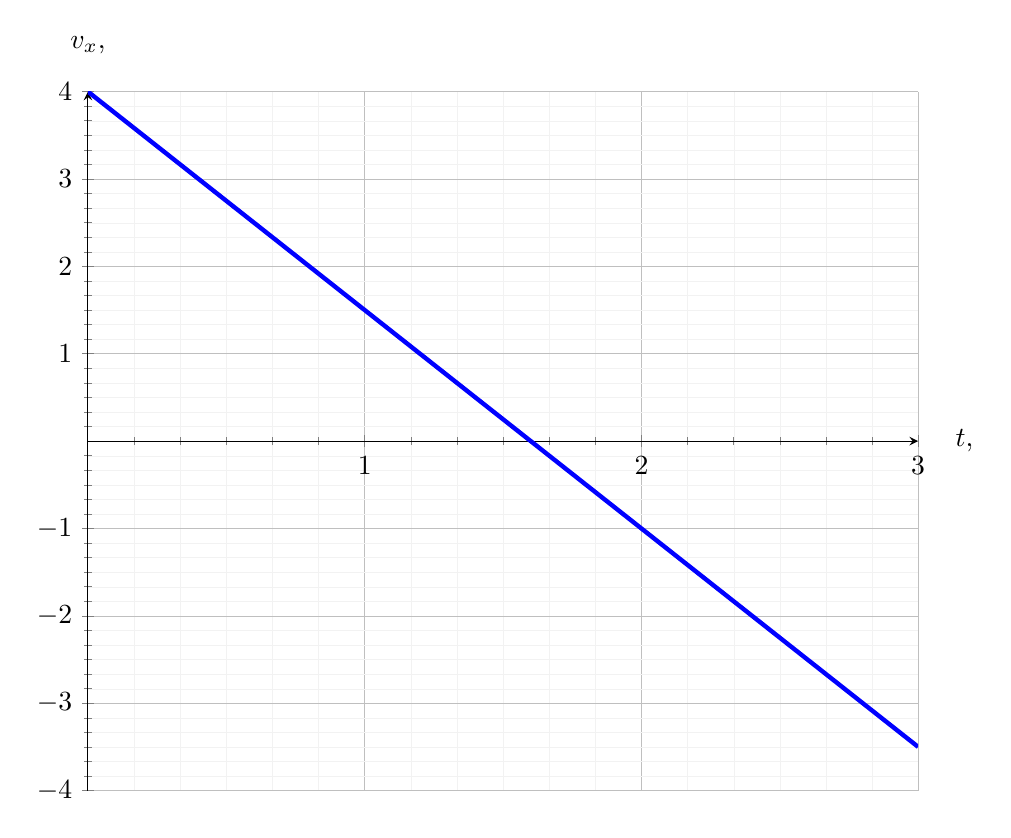
\begin{tikzpicture}
				\begin{axis}[%
					% === Налаштування сітки ===
					grid = both,
					grid style={line width=.1pt, draw=gray!10},
					major grid style={line width=.2pt,draw=gray!50},
					minor tick num = 5,
					minor grid style = {line width=.1pt,draw=gray!10},
					% === Налаштування положення координатних осей ===
					axis lines = middle,
					axis line style={-stealth},
					% === Вибір підписів шкали для відображення ===
					xtick = {0,1,...,4},
					ytick = {-4,...,4},
					% === Підпис координатних осей ===
					xlabel={$t$, \si{\second}},
					ylabel={$v_x$, \si{\meter\per\second}},
					% === Положення підпису координатних осей ===
					xlabel style={right = 10pt},
					ylabel style={above = 10pt},
					% === Налаштування мінімальних та максимальних значень координат ===
					xmin = 0,
					xmax =  3,
					ymin = -4,
					ymax =  4,
					% === Налаштування розміру графіка ===
					width=\linewidth,
					]
					\addplot+[blue, no marks, domain={0:3}, samples=100, ultra thick] {4 - 5/2*x};
					\end{axis}
				\end{tikzpicture}
				\caption{Problem~\ref{prb:ramp2}}
				\label{ramp2}
	\end{minipage}
	%---------------------------------------------------------
	\begin{minipage}[t]{0.45\linewidth}\centering
				\begin{tikzpicture}
				\tikzstyle{ground}=[fill,pattern=north east lines,draw=none,minimum width=2cm,minimum height=0.3cm]
				\node (wall1) [ground, minimum width=4cm,yshift=-0.15cm] {};
				\draw (wall1.north west) -- (wall1.north east);
				\fill[red!50, draw=black] (-1,0) rectangle +(2,2) [add reference=BP];
				\draw[-{Latex[open]}, thick, blue, double distance=1pt] (BP center) -- +(-40:3) node[right] {$\vec F$} ;
				\draw[dashed] (BP center) -- +(2,0);
				\draw (BP center) +(0:0.5) arc(0:-40:0.5) node[pos = 0.5, right] {$\alpha$};
				\end{tikzpicture}
		\caption{Problem~\ref{prb:block_friction}}
		\label{block_friction}
	\end{minipage}
	%---------------------------------------------------------
\end{figure}
%=========================================================


%=========================================================
\begin{problem}\label{prb:ushed_block}
	A $4.10$~kg block is pushed along a floor by a constant applied force that is horizontal and has a magnitude of $40.0$~N. Figure~\ref{ushed_block} gives the block’s speed $v$ versus time $t$ as the block moves along an $x$ axis on the floor. What is the coefficient of kinetic friction between the block and the floor?
\end{problem}


%=========================================================
\begin{problem}
	A $110$~g hockey puck sent sliding over ice is stopped in $15$~m by the frictional force on it from the ice.
	\begin{enumerate*}[label=(\alph*)]
		\item If its initial speed is $6.0$~m/s, what is the magnitude of the frictional force?
		\item What is the coefficient of friction between the puck and the ice?
	\end{enumerate*}
\end{problem}


%=========================================================
\begin{problem}
	A circular curve of highway is designed for traffic moving at $60$~km/h. Assume the traffic consists of cars without negative lift. 
	\begin{enumerate*}[label=(\alph*)]
		\item If the radius of the curve is $150$~m, what is the correct angle of banking of the road?
		\item If the curve were not banked, what would be the minimum coefficient of friction between tires and road that would keep traffic from skidding out of the turn when traveling at $60$~km/h? 
	\end{enumerate*}
\end{problem}


%=========================================================
\begin{problem}
	As a $40$~N block slides down a plane that is inclined at \ang{25} to the horizontal, its acceleration is $0.80$~\si{\meter\per\square\second}, directed up the plane. What is the coefficient of kinetic friction between the block and the plane?
	\begin{solution}
		$0.56$
	\end{solution}
\end{problem}


%=========================================================
\begin{problem}
	An initially stationary box of sand is to be pulled across a floor by means of a cable in which the tension should not exceed $1100$~N. The coefficient of static friction between the box and the floor is $0.35$. 
	\begin{enumerate*}[label = (\alph*)]
		\item What should be the angle between the cable and the horizontal in order to pull the greatest possible amount of sand, and
		\item  what is the weight of the sand and box in that situation?
	\end{enumerate*}
	\begin{solution}
		\begin{enumerate*}[label = (\alph*)]
			\item \ang{19},
			\item $3.3$~\si{\kilo\newton}.
		\end{enumerate*}
	\end{solution}
\end{problem}


%=========================================================
\begin{problem}\label{prb:body-rod-body}
	In Fig.~\ref{body-rod-body}, block 1 of mass $m_1 = 2.0$~kg and block 2 of mass $m_2 = 1.0$~kg are connected by a string of negligible mass. Block 2 is pushed by force of magnitude $20$~N and angle $\alpha = \ang{30}$. The coefficient of kinetic friction between each block and the horizontal surface is $0.20$. What is the tension in the string?
\end{problem}

%=========================================================
\begin{figure}[h!]\centering
	%---------------------------------------------------------
	\begin{minipage}[t]{0.45\linewidth}\centering
		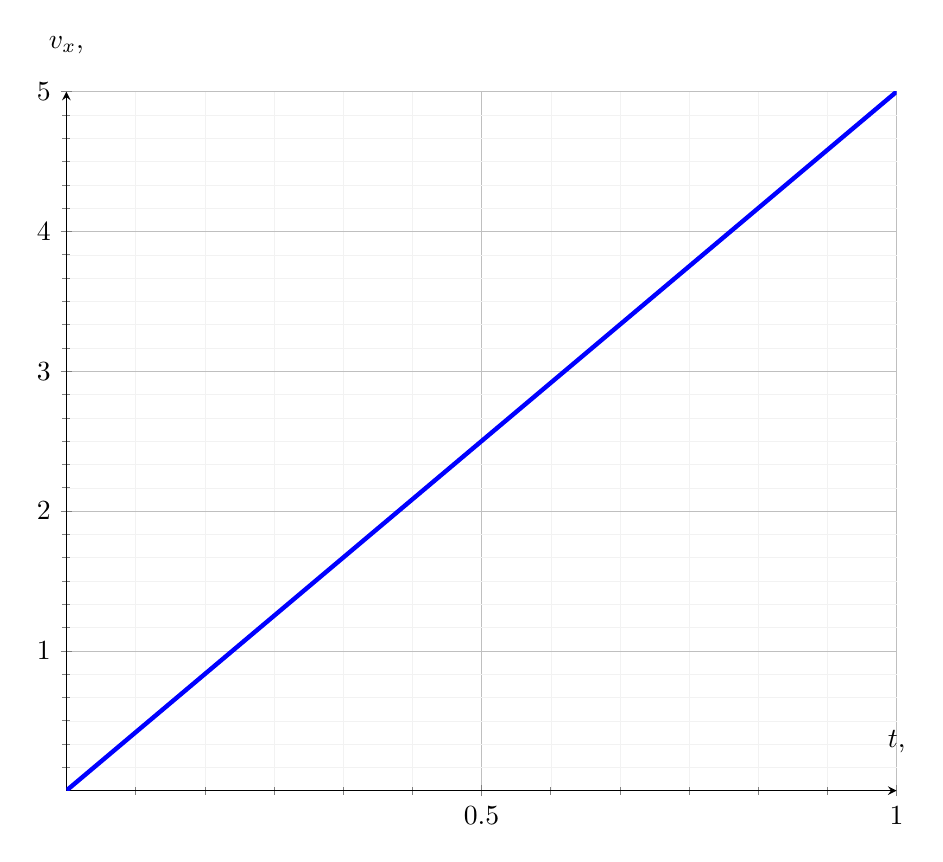
\begin{tikzpicture}
		\begin{axis}[%
		% === Налаштування сітки ===
		grid = both,
		grid style={line width=.1pt, draw=gray!10},
		major grid style={line width=.2pt,draw=gray!50},
		minor tick num = 5,
		minor grid style = {line width=.1pt,draw=gray!10},
		% === Налаштування положення координатних осей ===
		axis lines = middle,
		axis line style={-stealth},
		% === Вибір підписів шкали для відображення ===
		xtick = {0,0.5,1},
		ytick = {0,...,5},
		% === Підпис координатних осей ===
		xlabel={$t$, \si{\second}},
		ylabel={$v_x$, \si{\meter\per\second}},
		% === Положення підпису координатних осей ===
		xlabel style={above = 10pt},
		ylabel style={above = 10pt},
		% === Налаштування мінімальних та максимальних значень координат ===
		xmin = 0,
		xmax =  1,
		ymin = 0,
		ymax =  5,
		% === Налаштування розміру графіка ===
		width=\linewidth,
		]
		\addplot+[blue, no marks, domain={0:3}, samples=100, ultra thick] {5*x};
		\end{axis}
		\end{tikzpicture}
		\caption{Problem~\ref{prb:ushed_block}}
		\label{ushed_block}
	\end{minipage}
	%---------------------------------------------------------
	\begin{minipage}[t]{0.45\linewidth}\centering
			\begin{tikzpicture}
				\tikzstyle{ground}=[fill,pattern=north east lines,draw=none,minimum width=2cm,minimum height=0.3cm]
				\node (wall1) [ground, minimum width=8cm,yshift=-0.15cm] {};
				\draw (wall1.north west) -- (wall1.north east);
				\fill[red!50, draw=black] (-3,0) rectangle +(2,2) [add reference=BP1];
				\fill[blue!50, draw=black] (1.5,0) rectangle +(1.5,1.5) [add reference=BP2];
				\draw[thick] ([yshift=-0.25cm]BP1 east) -- (BP2 west);
				\draw[{Latex[open]-}, thick, blue, double distance=1pt] (BP2 north west) node[above right, black] {$\vec F$} -- +(135:2);
				\draw[dashed] (BP2 north west) -- +(-1,0);
				\draw (BP2 north west) +(180:0.5) arc (180:135:0.5) node[pos=0.5, left] {$\alpha$};
				\node at (BP1 center) {$m_1$};\node at (BP2 center) {$m_2$};
			\end{tikzpicture}
		\caption{Problem~\ref{prb:body-rod-body}}
		\label{body-rod-body}
	\end{minipage}
	%---------------------------------------------------------
\end{figure}
%=========================================================

\section{Dynamics of motion along a curved path}


%=========================================================
\begin{problem}\label{prb:car_on_hill}
	In Fig.~\ref{car_on_hill}, a car is driven at constant magnitude of velocity over a circular hill and then into a circular valley with the same radius. At the top of the hill, the normal force on the driver from the car seat is $0$. The driver’s mass is $70.0$~kg. What is the magnitude of the normal force on the driver from the seat when the car passes through the bottom of the valley?
	\begin{solution}
		$1.37 \cdot 10^3$~\si{\newton}.
	\end{solution}
\end{problem}

%---------------------------------------------------------
\begin{figure}[h!]\centering
	\begin{tikzpicture}
	\coordinate (C1) at (5,2);
	\coordinate (C2) at (10,0);
	\draw [thick, tangent=0.15, name path=A
	]  
	(0,0) ..controls (2,0) and (3,2).. (C1) 
	..controls (7,2) and (8,0).. (10,0)
	..controls (12,0) and (13,2).. (15,2)
	;
	\path [yshift=-0.2cm, name path=B
	]  
	(0,0) ..controls (2,0) and (3,2).. (5,2) 
	..controls (7,2) and (8,0).. (10,0)
	..controls (12,0) and (13,2).. (15,2)
	;
	\tikzfillbetween[of=A and B]{pattern=north west lines};
	\fill[red!50, draw=black, use tangent] (0,0) -- ++(0.5,0) -- ++(0,0.5) -- ++(-0.5,0) -- cycle;
	\draw[blue, -latex, thick, use tangent] (0.25,0.25) -- +(1,0) node[above right] {$\vec v$};
	\draw[dashed] ([yshift=-2cm]C1) circle (2);
	\draw[-latex] ([yshift=-2cm]C1) -- +(45:2) node[pos=0.5, above, rotate=45] {Radius};
	\draw[dashed] ([yshift=2cm]C2) circle (2);
	\draw[-latex] ([yshift=2cm]C2) -- +(-45:2) node[pos=0.5, above, rotate=-45] {Radius};
	\end{tikzpicture}
	\caption{Problem~\ref{prb:car_on_hill}}
	\label{car_on_hill}
\end{figure}
%---------------------------------------------------------



%=========================================================
\begin{problem}
	A ball suspended by a thread swings in a vertical plane so that its acceleration values in the extreme and the lowest position 
	are equal. Find the thread deflection angle in the extreme position. 
	\begin{solution}
		$\approx \ang{53}$.
	\end{solution}
\end{problem}


%%=========================================================
%\begin{problem}
%	A child of mass m swings in a swing supported by two
%	chains, each of length $R$. If the tension in each chain at
%	the lowest point is $T$, find 
%	\begin{enumerate*}[label=(\alph*)]
%		\item the child’s speed at the lowest point 
%		and
%		\item the force exerted by the seat on the child at the lowest point. (Ignore the mass of the seat.)
%	\end{enumerate*}
%	\begin{solution}
%		\begin{enumerate*}[label=(\alph*)]
%			\item $v = \sqrt{R\left( \frac{2T}{m} - g\right) }$,
%			\item $2T$.
%		\end{enumerate*}
%	\end{solution}
%\end{problem}


%=========================================================
\begin{problem}\label{prb:rotating_ball}
	A small sphere of mass $m$ is attached to the end of a cord of length $R$ and set into motion in a vertical circle about a fixed point $O$ as illustrated in Figure~\ref{rotating_ball}. Determine the tangential acceleration of the sphere and the tension in the cord at any instant when the velocity of the sphere is $v$ and the cord makes an angle $\theta$ with the vertical.
	\begin{solution}
		$T = mg \left( \frac{v^2}{gR} + \cos\theta\right) $
	\end{solution}
\end{problem}

%=========================================================
\begin{problem}\label{prb:conic_pendulum}
	Consider a conical pendulum (Fig.~\ref{conic_pendulum}) with a bob of mass $m = 80.0$~kg on a string of length $l = 10.0$~m that makes an angle of $\theta = \ang{5.00}$ with the vertical. Determine 
	\begin{enumerate*}[label=(\alph*)]
		\item the horizontal and vertical components of the force exerted by the string on the pendulum and
		\item the radial acceleration of the bob.
	\end{enumerate*}
\end{problem}

%=========================================================
\begin{figure}[h!]\centering
	%---------------------------------------------------------
		\begin{minipage}[t]{0.45\linewidth}\centering
		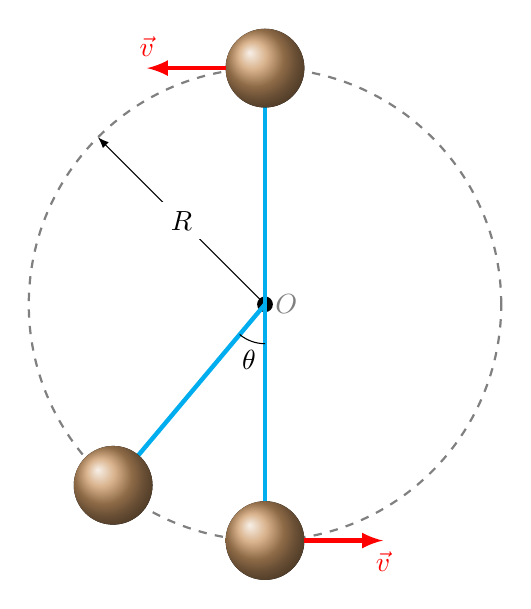
\begin{tikzpicture}
		\pgfmathsetmacro{\R}{3}
		\pgfmathsetmacro{\RB}{0.5}
		\pgfmathsetmacro{\bangle}{40}
		\coordinate (O) at (0,0);
		
		\coordinate (B1) at (90:\R);
		\coordinate (B2) at (270-\bangle:\R);
		\coordinate (B3) at (270:\R);
		
		\fill [] (O) circle (0.1);
		\draw[-latex] (O) -- +(135:\R) node[pos=0.5, fill=white] {$R$};
		\draw[ultra thick, cyan] (O) -- (B1);
		\draw[ultra thick, cyan] (O) -- (B2);
		\draw[ultra thick, cyan] (O) -- (B3);
		\draw[dashed, gray, thick] (O) circle (\R) node[right] {$O$};
		\fill[ball color = brown!80] (B1) circle (\RB);
		\fill[ball color = brown!80] (B2) circle (\RB);
		\fill[ball color = brown!80] (B3) circle (\RB);
		\draw[-latex, ultra thick, red] ([xshift=-\RB cm]B1) -- +(-1,0) node[above] {$\vec v$};
		\draw[-latex, ultra thick, red] ([xshift=\RB cm]B3) -- +(1,0) node[below] {$\vec v$};
		\draw (0,0) +(270:0.5) arc (270:270-\bangle:0.5) node[pos=0.6, below] {$\theta$};
		\end{tikzpicture}
		\caption{Problems~\ref{prb:rotating_ball}}
		\label{rotating_ball}
	\end{minipage}
	%---------------------------------------------------------
	\begin{minipage}[t]{0.45\linewidth}\centering
	\begin{tikzpicture}
		\pgfmathsetmacro{\pangle}{30}
		\pgfmathsetmacro{\l}{5}
		\tikzstyle{ground}=[fill,pattern=north east lines,draw=none,minimum width=2cm,minimum height=0.3cm]
		\node (wall) [ground, minimum width=1cm,yshift=0.15cm] {};
		\draw (wall.south west) -- (wall.south east);
		\draw[dashed] (0,0) -- +(270:{\l*cos(\pangle)}) coordinate (E);
		\draw[ultra thick, cyan] (0,0) -- (270-\pangle:\l) coordinate (B);
		\fill[ball color = brown] (B) circle (0.5);
		\draw (0,0) +(270:0.5) arc (270:{270-\pangle}:0.5) node[pos=0.8, below] {$\theta$};
		\draw[dashed] (E) ellipse ({\l*sin(\pangle)} and 0.5);
		\node[pt=black] at (0,0) {};
	\end{tikzpicture}
	\caption{Problem~\ref{prb:conic_pendulum}}
	\label{conic_pendulum}
	\end{minipage}
	%---------------------------------------------------------
\end{figure}
%=========================================================

%=========================================================
\begin{problem}\label{prb:sliding_from_sphere}
	\addpic{2}{0.3\linewidth}{%
	\centering	
	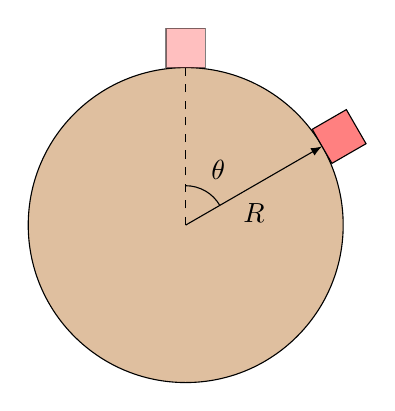
\begin{tikzpicture}
		\pgfmathsetmacro{\R}{2}
		\pgfmathsetmacro{\bang}{30}
		\draw[fill=brown!50] (0,0) circle (\R);
		\draw[dashed] (0,0) -- (0,\R);
		\draw[-latex] (0,0) -- +(\bang:\R) node[pos=0.5, below = 0.1cm] {$R$};
		\draw[] (0,0) +(90:0.5) arc (90:\bang:0.5) node[pos=0.4, above right] {$\theta$};
		\draw[fill=red!50, opacity=0.5] (-0.25,\R) rectangle +(0.5,0.5);
		\draw[fill=red!50, rotate = {\bang-90}] (-0.25,\R) rectangle +(0.5,0.5);
	\end{tikzpicture}
	\captionof{figure}{Problem~\ref{prb:sliding_from_sphere}}
	\label{sliding_from_sphere}
	}
	A small body $A$ starts sliding off the top of a smooth sphere 
	of radius $R$ (Fig.~\ref{sliding_from_sphere}). Find 
	\begin{enumerate*}[label = (\alph*)]
		\item the angle $\theta$  corresponding to the point 
		at which the body breaks off the sphere and
		\item  the break-of velocity of the body.
	\end{enumerate*}
	\begin{solution}
		\begin{enumerate*}[label = (\alph*)]
			\item $\theta = \arccos\frac23 $,
			\item $v = \sqrt{\frac{2}{3}gR}$. 
		\end{enumerate*}
	\end{solution}
\end{problem}

\Closesolutionfile{answer}

